\chapter{Ejercicio teleoperador acústico y banda sonora}\label{audio}
En este capítulo se nombran las herramientas utilizadas y cómo se ha realizado el ejercicio del teleoperador acústico, que aborda el análisis de audio de entrada. También se muestra cómo se ha añadido la posibilidad de incluir efectos de sonido y bandas sonoras (audio de salida) a los ejercicios ya existentes.

La entrada y salida de audio desde aplicaciones web es muy interesante para conseguir una mayor interactividad con el usuario. El sonido es muy importante en el mundo real y llevarlo a la Websim nos permite que la simulación sea más inmersiva y la experiencia el usuario sea más agradable.
 El audio de entrada o \textit{audio in} en este trabajo  lo vamos a utilizar para coger las muestras del micrófono y analizarlo  para reconocer las palabras que entiende nuestro robot y  actué de forma adecuada. El audio de salida o \textit{audio out} se usará para completar los ejercicios con bandas sonoras y el sonido de colisión.

\section{Enunciado}  
En este ejercicio se va a desarrollar un teleoperador acústico. El objetivo es crear un algoritmo de reconocimiento de voz con JavaScript, para poder dirigir un robot de Kibotics con la voz.

El alumno deberá indicarle  al robot órdenes claras para que él reconozca cada orden  y pueda moverse por el escenario. Hay dos escenarios disponibles, un muro de piedra y una portería de rugby. El robot elegido es un dron que deberá moverse por el mundo sin chocar con ellos.

\section{Modelos del mundo }
Para empezar con este ejercicio se utilizó un fichero de configuración sencillo en el que sólo aparece un dron y un plano con una textura de césped. Este fichero es necesario para que el simulador Websim construya la escena 3D. 
Ésta sería una parte de ese fichero donde se muestra la configuración de la escena \textit{(scene)}, los robots \textit {(robots\_config)}, las texturas \textit{(assets)} y los objetos \textit{(objects)}.

\begin{lstlisting}
{
    "scene-parent-id": "myIFrame",
    "scene": {
        "id": "scene",
        "gravity": 0,
        "sky": "../../assets/textures/sky.png",
        "background": "color: gray;",
        "inspector": "url: https://aframe.io/releases/0.4.0/aframe-inspector.min.js",
        "embedded": true,
        "physics": "debug: true"
    },
    "robots_config": [
        {
            "controller": "user1",
            "id": "a-pibot"
        }
    ],
    "assets": [
        {
            "tag": "img",
            "attr": {
                "id": "ground",
                "alt": "Texture for the scene ground",
                "src": "../../assets/textures/escenarioLiso-min.png"
            }
       ],
    "objects":[
     
        {
            "tag": "a-plane",
            "attr": {
                "static-body": {
                    "mass": 100000
                },
                "position": { "x":0, "y":0, "z":0 },
                "rotation": { "x":-90, "y":0, "z":0 },
                "width": "100",
                "height": "100",
                "src":"#ground"
            }
        },
        {
            "tag": "a-robot",
            "attr": {
                "id": "a-pibot",
                "gltf-model":"../../assets/models/drone_animation.gltf",
                "scale": { "x":0.5, "y":0.5, "z":0.5},
                "position": { "x":0, "y":4, "z":0},
                "rotation": { "x":0, "y":90, "z":0},
                "dynamic-body":{"mass": 1}

            },      
  }
\end{lstlisting}


Para este ejercicio se crearon dos escenarios: uno con portería de rugby y otro con una pared, que se añadieron al  fichero de configuración anterior. La portería se creó con Blender y la pared con A-Frame en el fichero de configuración de Websim. Ver Figura 6.1 y 6.2.

 \begin{figure}[H]
  \begin{subfigure}[b]{0.5\textwidth}
  \centering
    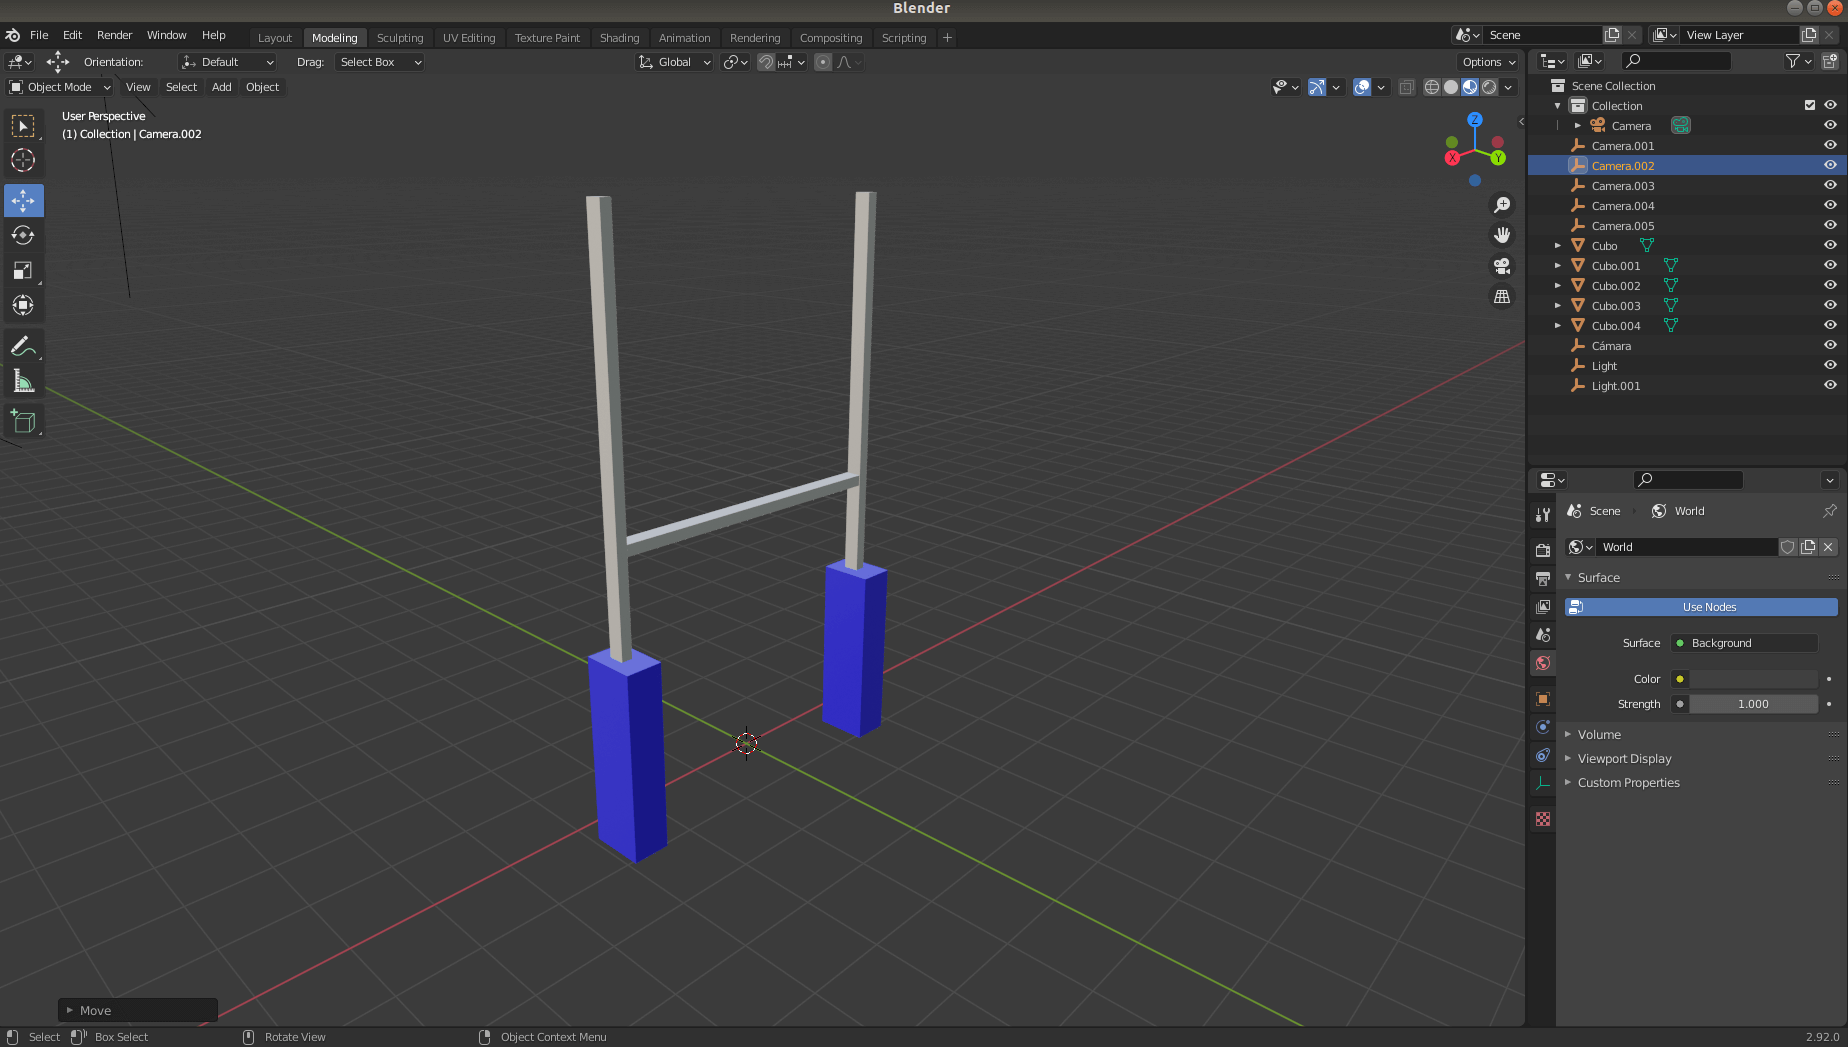
\includegraphics[width=0.95\textwidth, height=0.7\textwidth]{chapters/images/porteriablender.png}
    \caption{}
    \label{fig:f1}
  \end{subfigure}
  \hfill
  \begin{subfigure}[b]{0.5\textwidth}
  \centering
    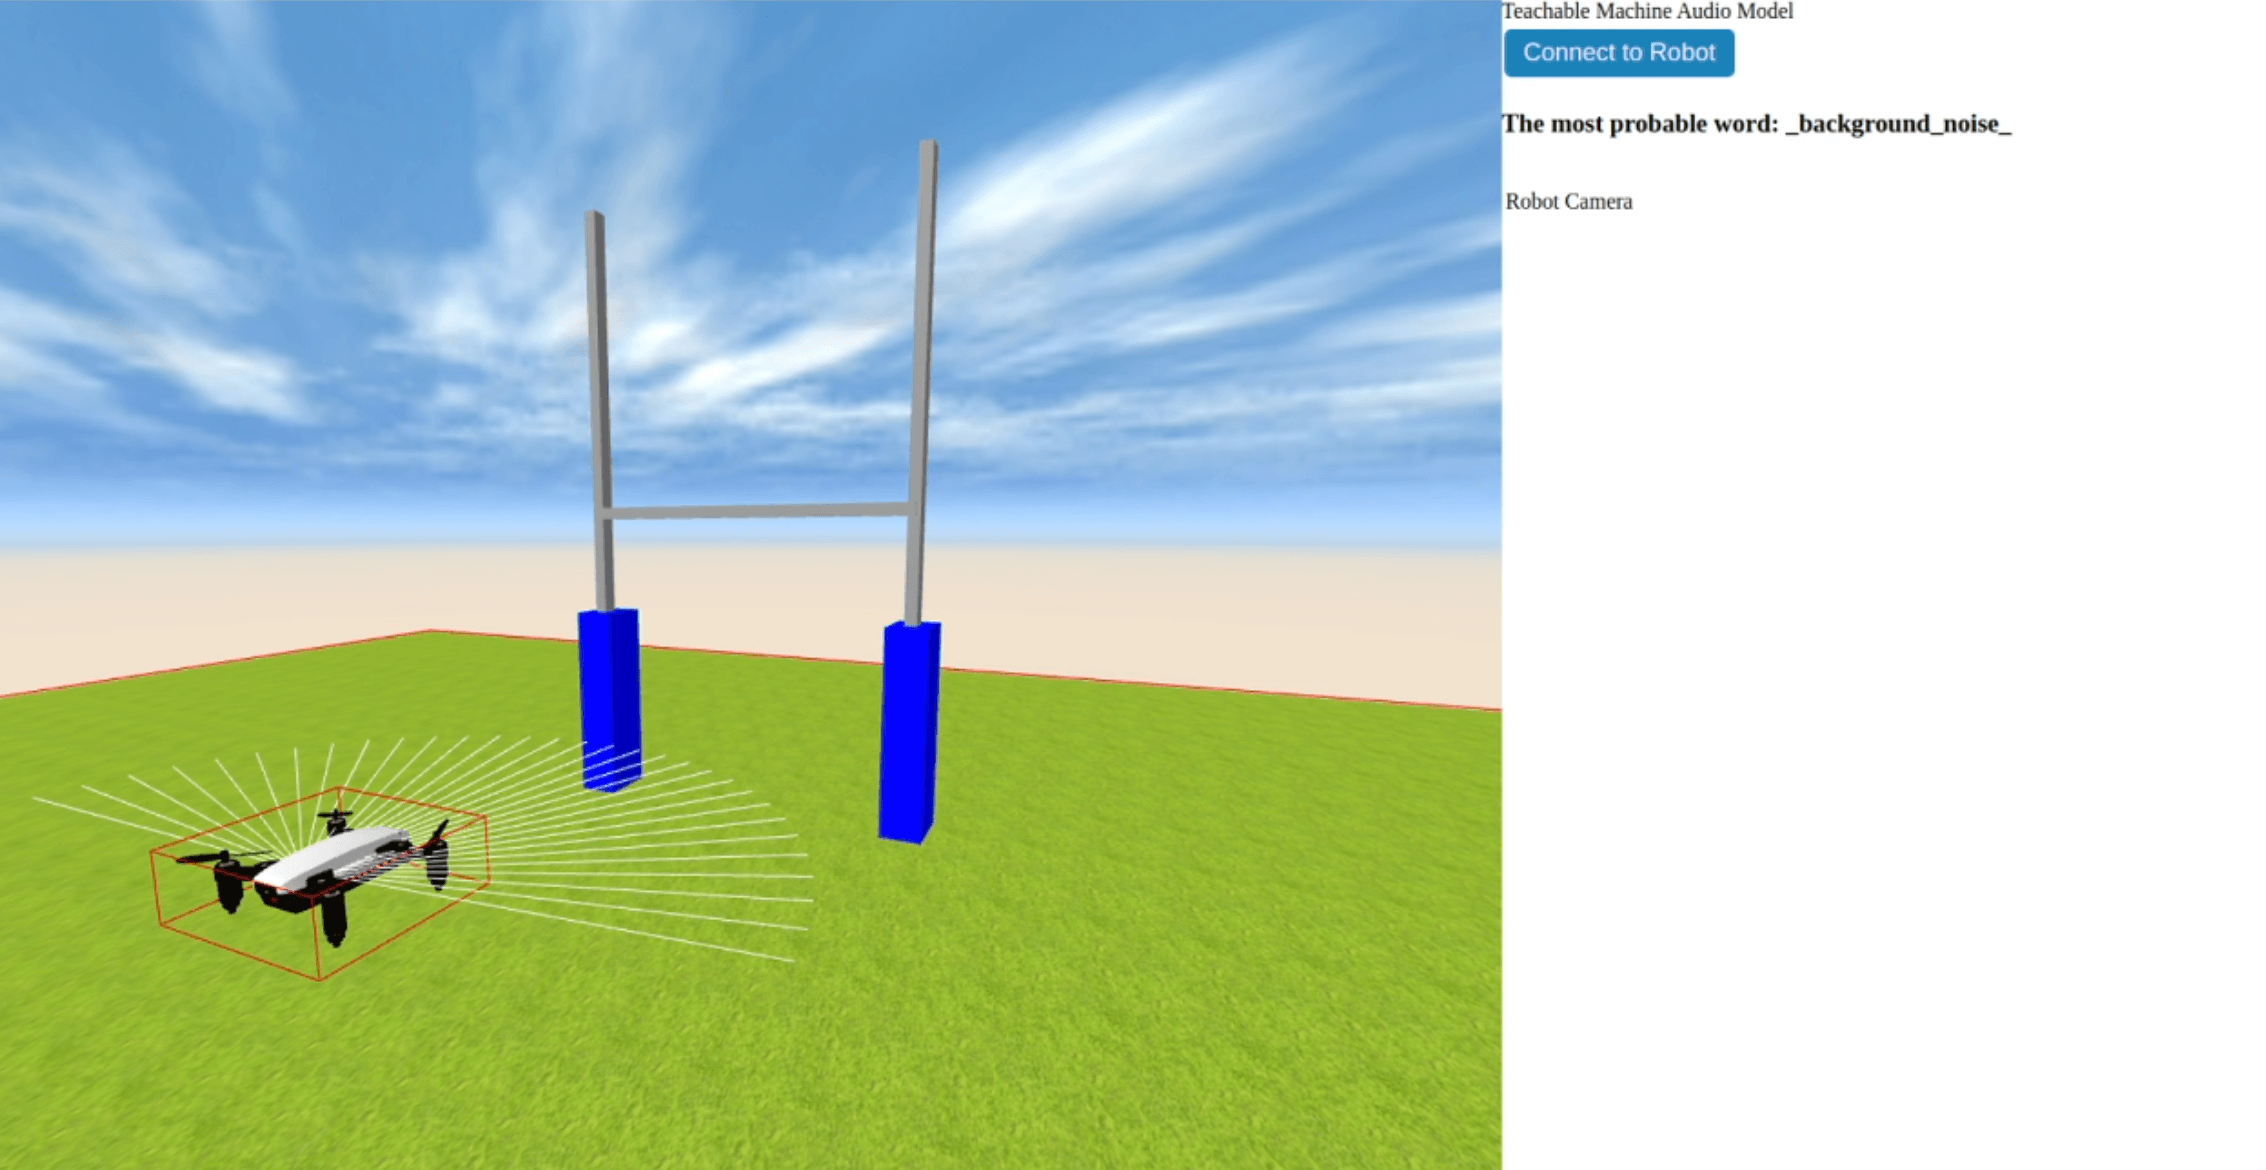
\includegraphics[width=0.95\textwidth, height=0.7\textwidth]{chapters/images/porteriawebsim.png}
	\caption{}    
    \label{fig:f2}
 
  \end{subfigure}
  \caption{Modelos portería en Blender y  en Websim }
\end{figure}


\begin{figure}[H]
\centering
    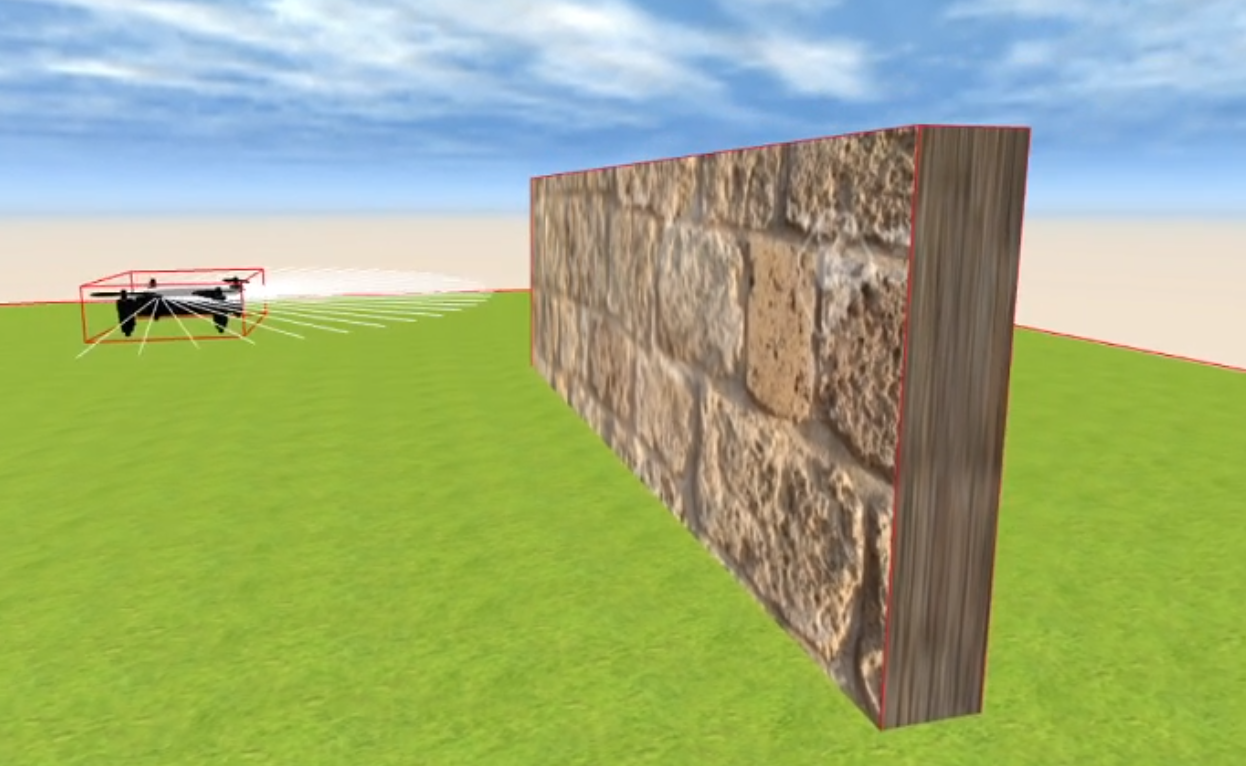
\includegraphics[width=0.7\textwidth, height=0.5\textwidth]{chapters/images/pared.png}
    \caption{Pared de piedra en Websim}
    \label{fig:f1}
  \end{figure}

Estos modelos se han añadido al fichero de configuración de la siguiente forma:
\begin{lstlisting}
...
    "assets": [

        {
            "tag": "a-asset-item",
            "attr": {
                "id": "porteria_rugby"
		},
		
		{
            "tag": "img",
            "attr": {
                "id": "wall",
                "alt": "Texture for the scene wall",
                "src": "../../assets/textures/wall.jpg"}
        }
		...
    ],
    "objects":[ 
        {
            "tag": "a-entity",
            "attr": {
              "id":"porteria_rugby",
              "gltf-model":"../../assets/models/porteria_rugby.glb",
              "position": { "x":0, "y":0, "z":-15},
              "scale": { "x":3, "y":3, "z":3}

            }
        }
               {
            "tag":"a-box",
            "attr": {
                "id": "wall",
                "width": "30",
                "height": "20",
                "depth":"2",
                "position": { "x":0, "y":0, "z":-15},
                "src":"#wall",
                "static-body": {
                    "mass": 1
                }
            }
        },
...
  
\end{lstlisting}




\section{Procesamiento de audio con Teachable Machine}

El procesamiento de audio es muy complejo y existen muchas herramientas diferentes para implementarlo desde JavaScript. En este trabajo se han investigado tres herramientas y finalmente se ha decidido usar Teachable Machine, que es una herramienta basada en la Web para crear modelos de aprendizaje automático. Destaca por modelos de clasificación de imágenes, sonidos y posturas. Teachable Machine internamente usa TensorFlowJS . 

La creación de un modelo en Teachable Machine tiene 3 fases: recopilación, entrenamiento y exportación del modelo a tu proyecto.

\begin{itemize}
\item \textit{Recopilación :}

Para hacer el modelo primero hay que recopilar muestras. Para ello fue necesaria la participación de 10 personas para que el modelo generado fuera más completo y pudiera reconocer la palabra independientemente de si la voz del usuario es más aguda o más grave.  Se usaron aproximadamente 10 muestras de cada palabra por persona. El modelo cuenta con 105 muestras por cada palabra (10 muestras aproximadamente x 10 personas). Las palabras que queremos reconocer son \textit{go, stop, back, right, left, up, down } y el ruido de fondo. Esto ha supuesto un total de 840 muestras.

Las muestras se grabaron una a una en la página de creación de modelos de Teachable Machine. En la Figura 6.3 se puede ver el modelo y las muestras grabadas.


\begin{figure}[H]
 \centering
    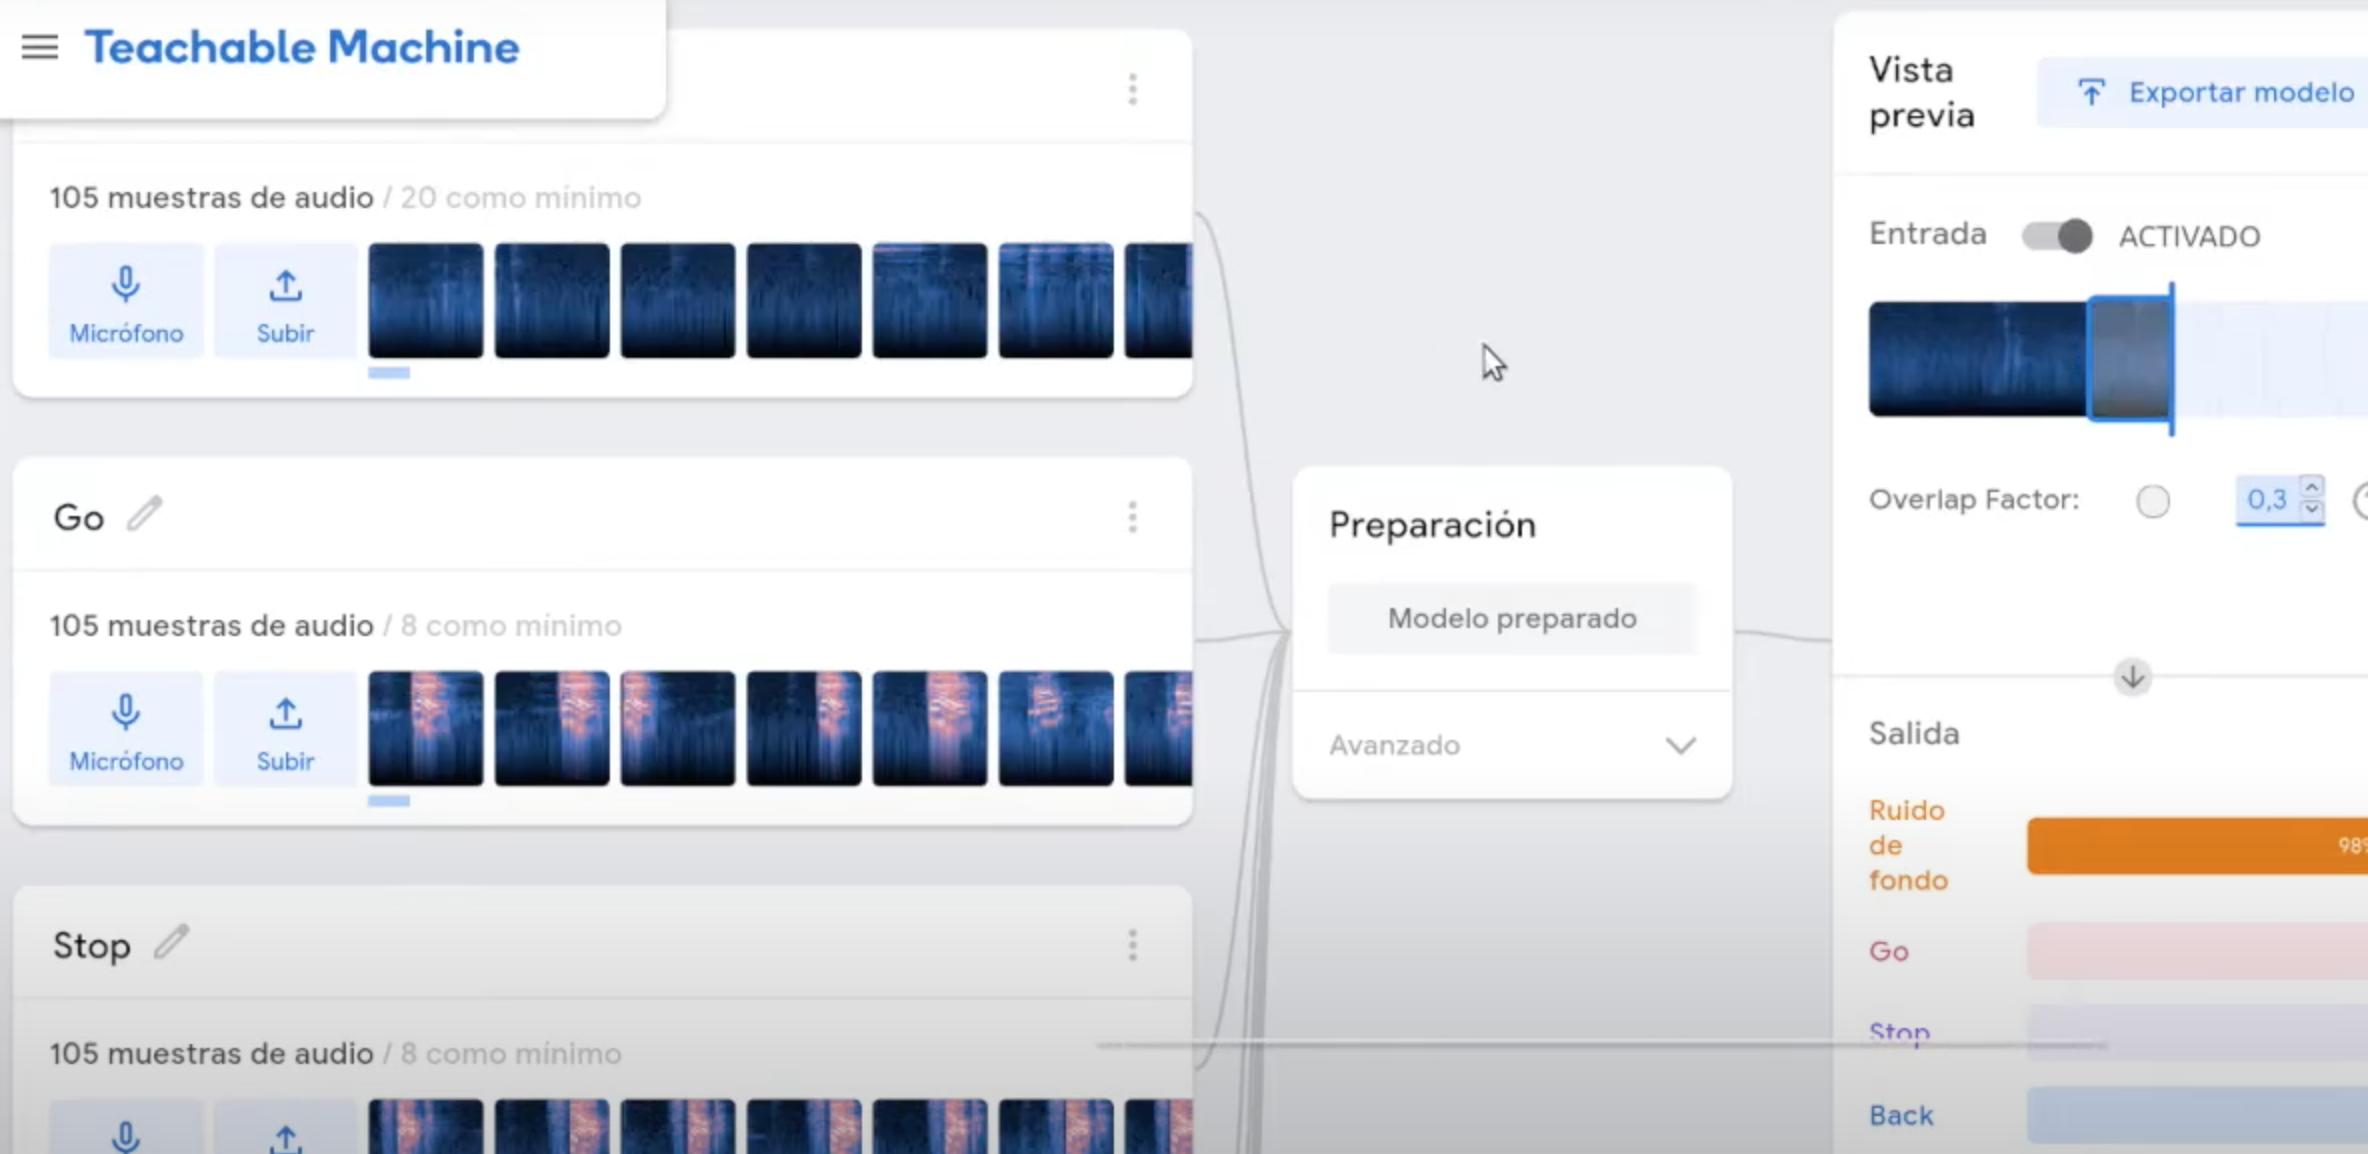
\includegraphics[width=0.8\textwidth, height=0.4\textwidth]{chapters/images/teachablemachine.png}
    \caption{Modelo realizado en Teachable Machine}
\end{figure}
 

\item  \textit{Entrenamiento :}

Una vez conseguidas todas las muestras, hay que entrenar el modelo, que se hace en `épocas'. Teachable Machine permite cambiarlas. Gracias a unas tablas de precisión y pérdidas por época puedes guiarte para que en función de tus datos puedas ajustar este parámetro. Para este proyecto se utilizaron los valores predeterminados, los cuales proporcionaron buenos resultados.

\item  \textit{Exportación del modelo a Websim :}

Una vez entrenado, la página web de Teachable Machine muestra una vista previa en el que puedes probar y ver el porcentaje de aciertos de cada palabra y con esto decidir si necesitas añadir más muestras o cambiar los parámetros de tu modelo.  En la Figura 6.4 podemos ver la visualización de prueba.

\begin{figure}[H]
 \centering
    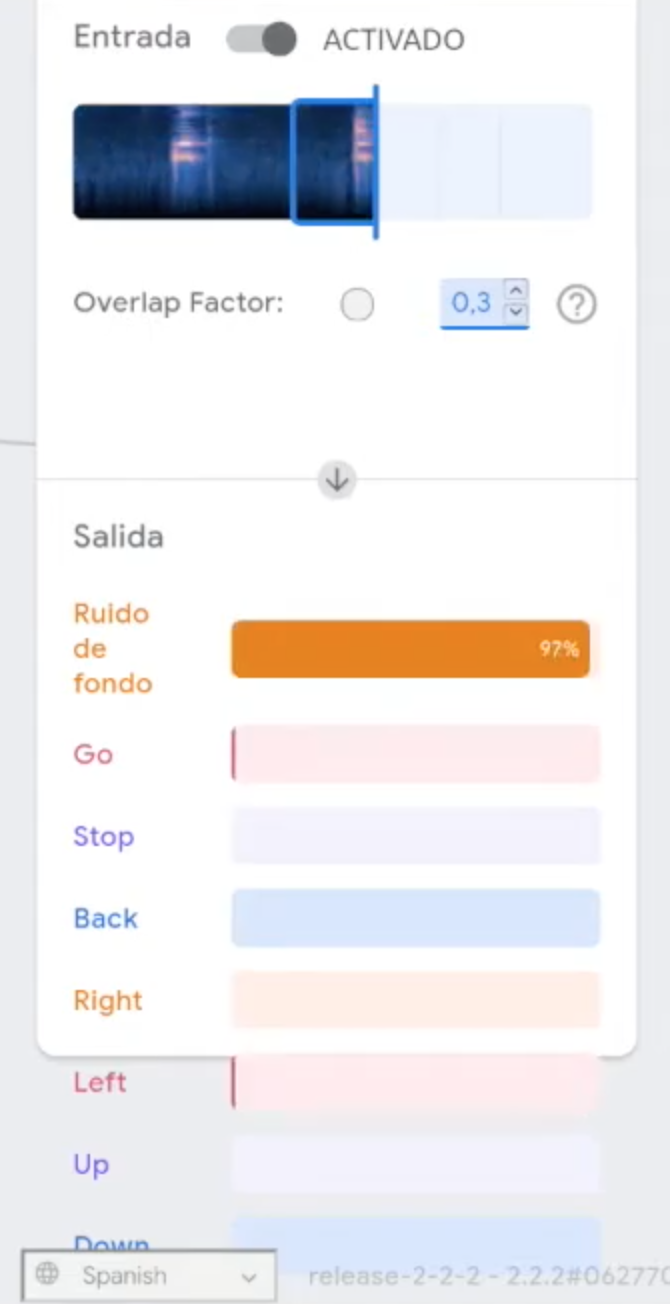
\includegraphics[width=0.4\textwidth, height=0.6\textwidth]{chapters/images/teachablemachine2.png}
    \caption{Vista previa del modelo}
\end{figure}
 

Una vez ajustado y con las 105 muestras por palabra, se exportó el modelo. 
Para exportarlo, Teachable Machine puede alojarlo en sus servidores y proporcionarte  un enlace de forma gratuita o puedes descargarlo. Se optó por guardarlo en la nube de Teachable Machine para que no ocupara mucho espacio en Kibotics, ya que la forma de importarlo  a JavaScript era similar en ambas opciones.
Una vez subido a la nube, Teachable Machine proporciona una URL de la dirección de tu modelo y el código necesario para importarlo a tu proyecto desde JavaScript.
\end{itemize}

Con estos 3 pasos ya tenemos creado nuestro modelo en Teachable Machine. Para probar el funcionamiento de este modelo se hizo una  primera prueba de reconocimiento de audio en una página web propia y específica, todavía sin fusionarlo con el comportamiento del robot en Websim. En este enlace \footnote{https://martaquintana.github.io/Audio\_Recognition/index.html} se puede probar el funcionamiento de este código basado en HTML5, CSS3, JavaScript y Teachable Machine(TensorFlowJS) (Ver Figura 6.5). Esta página web pide permiso para acceder al micrófono y, cuando lo tiene, analiza el audio  y muestra la probabilidad de cada palabra en tiempo real.  

Este es el código de esa página web de prueba del modelo, que incluye el código que nos facilita Teachable Machine a la hora de exportar el modelo:

\begin{lstlisting}
<html>
<head>
  <script src="https://cdn.jsdelivr.net/npm/@tensorflow/tfjs@1.3.1/dist/tf.min.js"></script>
  <script src="https://cdn.jsdelivr.net/npm/@tensorflow-models/speech-commands@0.4.0/dist/speech-commands.min.js"></script>
  <style type="text/css">
    button{
      text-decoration: none;
      padding: 10px;
      font-weight: 600;
      font-size: 20px;
      color: #ffffff;
      background-color: #AAA;
      border-radius: 6px;
      border: 2px solid black;
    }
    button:hover{
      color: black;
      background-color: #ffffff;
    }
    button:active {
    box-shadow: 0 2px #666;
    transform: translateY(2px);
  }

  </style>
</head>
<body>

<div>Teachable Machine Audio Model</div>
<button type="button" onclick="init()">Start</button>
<h3 id = "prediction" > The most probable word: </h3>
<div  id="label-container"  style="background-color: #D3D3D3;"></div>

<script type="text/javascript">
    // more documentation available at
    // https://github.com/tensorflow/tfjs-models/tree/master/speech-commands

    // the link to your model provided by Teachable Machine export panel
    const URL = "https://teachablemachine.withgoogle.com/models/P3XdF5r5d/";

    async function createModel() {
        const checkpointURL = URL + "model.json"; // model topology
        const metadataURL = URL + "metadata.json"; // model metadata

        const recognizer = speechCommands.create(
            "BROWSER_FFT", // fourier transform type, not useful to change
            undefined, // speech commands vocabulary feature, not useful for your models
            checkpointURL,
            metadataURL);

        // check that model and metadata are loaded via HTTPS requests.
        await recognizer.ensureModelLoaded();

        return recognizer;
    }

    async function init() {
        const recognizer = await createModel();
        const classLabels = recognizer.wordLabels(); // get class labels
        const labelContainer = document.getElementById("label-container");
        const word = document.getElementById("prediction");
        for (let i = 0; i < classLabels.length; i++) {
            labelContainer.appendChild(document.createElement("div"));
        }

        // listen() takes two arguments:
        // 1. A callback function that is invoked anytime a word is recognized.
        // 2. A configuration object with adjustable fields
        recognizer.listen(result => {
            const scores = result.scores; // probability of prediction for each class
            var word_index = 0;
            // render the probability scores per class
            for (let i = 0; i < classLabels.length; i++) {
                const classPrediction = classLabels[i] + ": " + result.scores[i].toFixed(2);
                labelContainer.childNodes[i].innerHTML = classPrediction;
                //The most probable word
                if (result.scores[i].toFixed(2) >= result.scores[word_index].toFixed(2)) {
                   word_index = i;

                }
            }
            var prediction = classLabels[word_index];
            word.innerHTML = "The most probable word: " + prediction;
            //console.log(prediction);
        }, {
            includeSpectrogram: true, // in case listen should return result.spectrogram
            probabilityThreshold: 0.75,
            invokeCallbackOnNoiseAndUnknown: true,
            overlapFactor: 0.50 // probably want between 0.5 and 0.75. More info in README
        });

        // Stop the recognition in 5 seconds.
        // setTimeout(() => recognizer.stopListening(), 5000);
    }
</script>
</<body>
</html>

\end{lstlisting}


\begin{figure}[H]
    \centering
    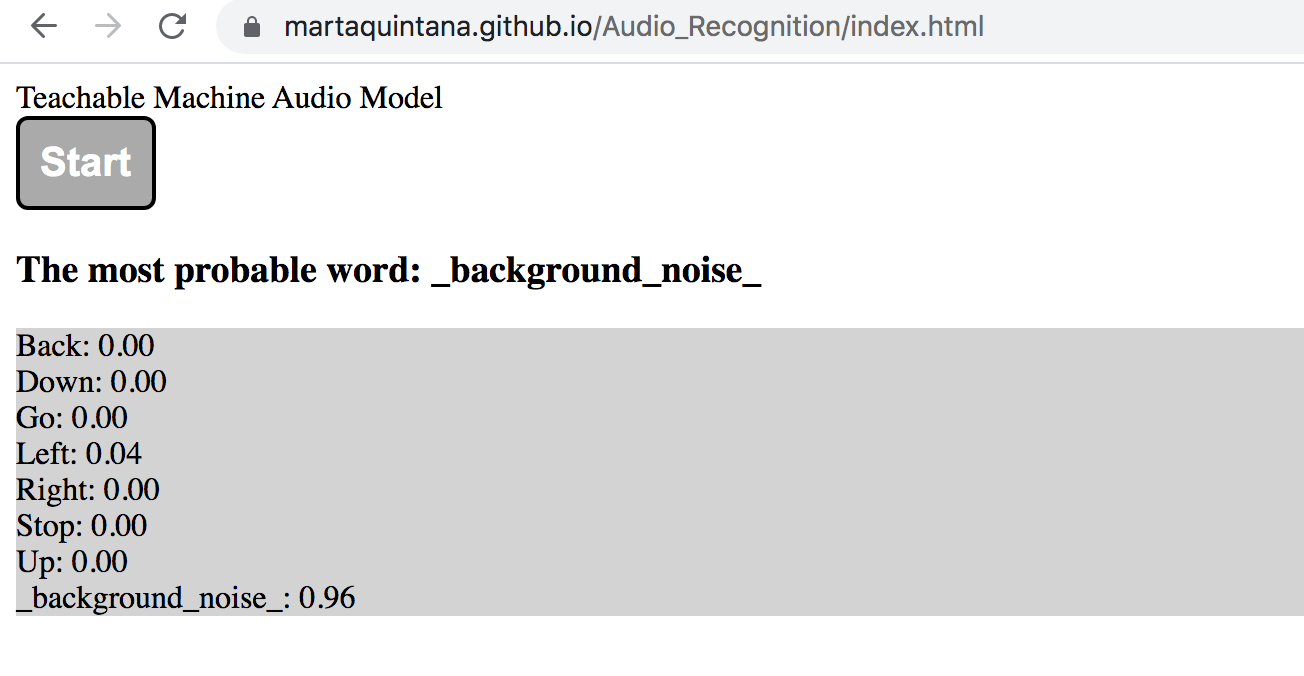
\includegraphics[width=0.8\textwidth, height=0.4\textwidth]{chapters/images/audioprueba.png}
    \caption{Página web de prueba de reconocimiento de audio}
    \label{fig:my_label}
\end{figure}

Una vez se comprobó que el modelo de reconocimiento de audio funcionaba satisfactoriamente, se incorporó a Websim. Para ello, se creó el siguiente fichero audio.js que se importa en el HTML del ejercicio de la siguiente forma:   

\begin{lstlisting}
<script type="text/javascript" src="js/audio.js" >
\end{lstlisting}

Código de audio.js:

\begin{lstlisting}
document.addEventListener('robot-loaded', (evt)=>{
  localRobot = evt.detail;
  console.log(localRobot);
});
// more documentation available at
// https://github.com/tensorflow/tfjs-models/tree/master/speech-commands

// the link to your model provided by Teachable Machine export panel
const URL = "https://teachablemachine.withgoogle.com/models/P3XdF5r5d/";
var connection = false;
var noise_times = 0;

async function createModel() {
    const checkpointURL = URL + "model.json"; // model topology
    const metadataURL = URL + "metadata.json"; // model metadata

    const recognizer = speechCommands.create(
        "BROWSER_FFT", // fourier transform type, not useful to change
        undefined, // speech commands vocabulary feature, not useful for your models
        checkpointURL,
        metadataURL);

    // check that model and metadata are loaded via HTTPS requests.
    await recognizer.ensureModelLoaded();

    return recognizer;
}

async function analizar(recognizer,classLabels,word) {
//  for (let i = 0; i < classLabels.length; i++) {
  //    labelContainer.appendChild(document.createElement("div"));
  //}

  // listen() takes two arguments:
  // 1. A callback function that is invoked anytime a word is recognized.
  // 2. A configuration object with adjustable fields
  recognizer.listen(result => {
      console.log(noise_times)
      const scores = result.scores; // probability of prediction for each class
      var word_index = 0;

      // render the probability scores per class
      for (let i = 0; i < classLabels.length; i++) {
          const classPrediction = classLabels[i] + ": " + result.scores[i].toFixed(2);
          //labelContainer.childNodes[i].innerHTML = classPrediction;
          //The most probable word
          if (result.scores[i].toFixed(2) >= result.scores[word_index].toFixed(2)) {
             word_index = i;
          }
      }
      var prediction = classLabels[word_index];
      word.innerHTML = "The most probable word: " + prediction;
      if (String(prediction) == "_background_noise_"){
        noise_times = noise_times + 1;
      }else{
        noise_times = 0;
      }
      if (connection){
        if (String(prediction) == "Go") {
          localRobot.setV(0.9);
          //que se mueva el robot
        }else if (String(prediction) == "Stop") {
           localRobot.setV(0);
           localRobot.setW(0);
           localRobot.setL(0);
          //que se pare
        }else if (String(prediction) == "Back"){
           localRobot.setV(-0.9);
        }else if (String(prediction) == "Right"){
            localRobot.setW(-0.005);

        }else if (String(prediction) == "Left"){
            localRobot.setW(0.005);

        }else if (String(prediction) == "Up"){
            localRobot.setL(0.25);

        }else if (String(prediction) == "Down"){
            noise_times = 0;
            console.log(localRobot.velocity);
            if (localRobot.velocity.y = 0.25) {
              localRobot.setL(-0.25);
            }
        }
        //For stop going down or going up, turn left or turn right say the word : STOP

      }
      //console.log(prediction);
  }, {
      includeSpectrogram: true, // in case listen should return result.spectrogram
      probabilityThreshold: 0.75,
      invokeCallbackOnNoiseAndUnknown: true,
      overlapFactor: 0.50 // probably want between 0.5 and 0.75. More info in README
  });

  // Stop the recognition in 10 seconds.
  setTimeout(() => {recognizer.stopListening(); }, 10000);

}

async function listen() {
        document.getElementById("listen_again").style.visibility = 'hidden';
        //--------TEACHABLE MACHINE--------------
        const recognizer = await createModel();
        const classLabels = recognizer.wordLabels(); // get class labels
        //const labelContainer = document.getElementById("label-container");
        const word = document.getElementById("prediction");
      //  for (let i = 0; i < classLabels.length; i++) {
        //    labasync function listen() {elContainer.appendChild(document.createElement("div"));
        //}

       var id = setInterval(() => {if(noise_times <= 10){analizar(recognizer,classLabels,word)}else{
          setTimeout(() => {console.log("Se ha parado de analizar")
            word.innerHTML = "The most probable word: " ;
            clearInterval(id);
            document.getElementById("listen_again").style.visibility = 'visible';
            //Robot Control opcional
            //localRobot.setV(0);
            //localRobot.setW(0);
            //localRobot.setL(0);
          }, 10000);
        }}, 10150);

}

async function Back\_To\_Listen(){
   document.getElementById("prediction").innerHTML= 'The most probable word: <br> <img src="https://wbl.telcel\-id.com:8443/images/Load\_Icon.gif" alt="Loading the model">'
   noise\_times = 0;
   listen();
}

async function Connect\_To\_Robot() {
    if (connection){connection= false;
      document.getElementById("connection").style.backgroundColor= "red";
      console.log( "Desconectado");
    }else{
        connection = true;
        listen();
        console.log( "CONECTADO AL ROBOT");
        document.getElementById("connection").style.backgroundColor= "green";
    }
}
\end{lstlisting}

Con el fichero de configuración, el HTML y este código JavaScript el ejercicio se visualiza como se muestra en la Figura 6.6.

\begin{figure}[H]
    \centering
    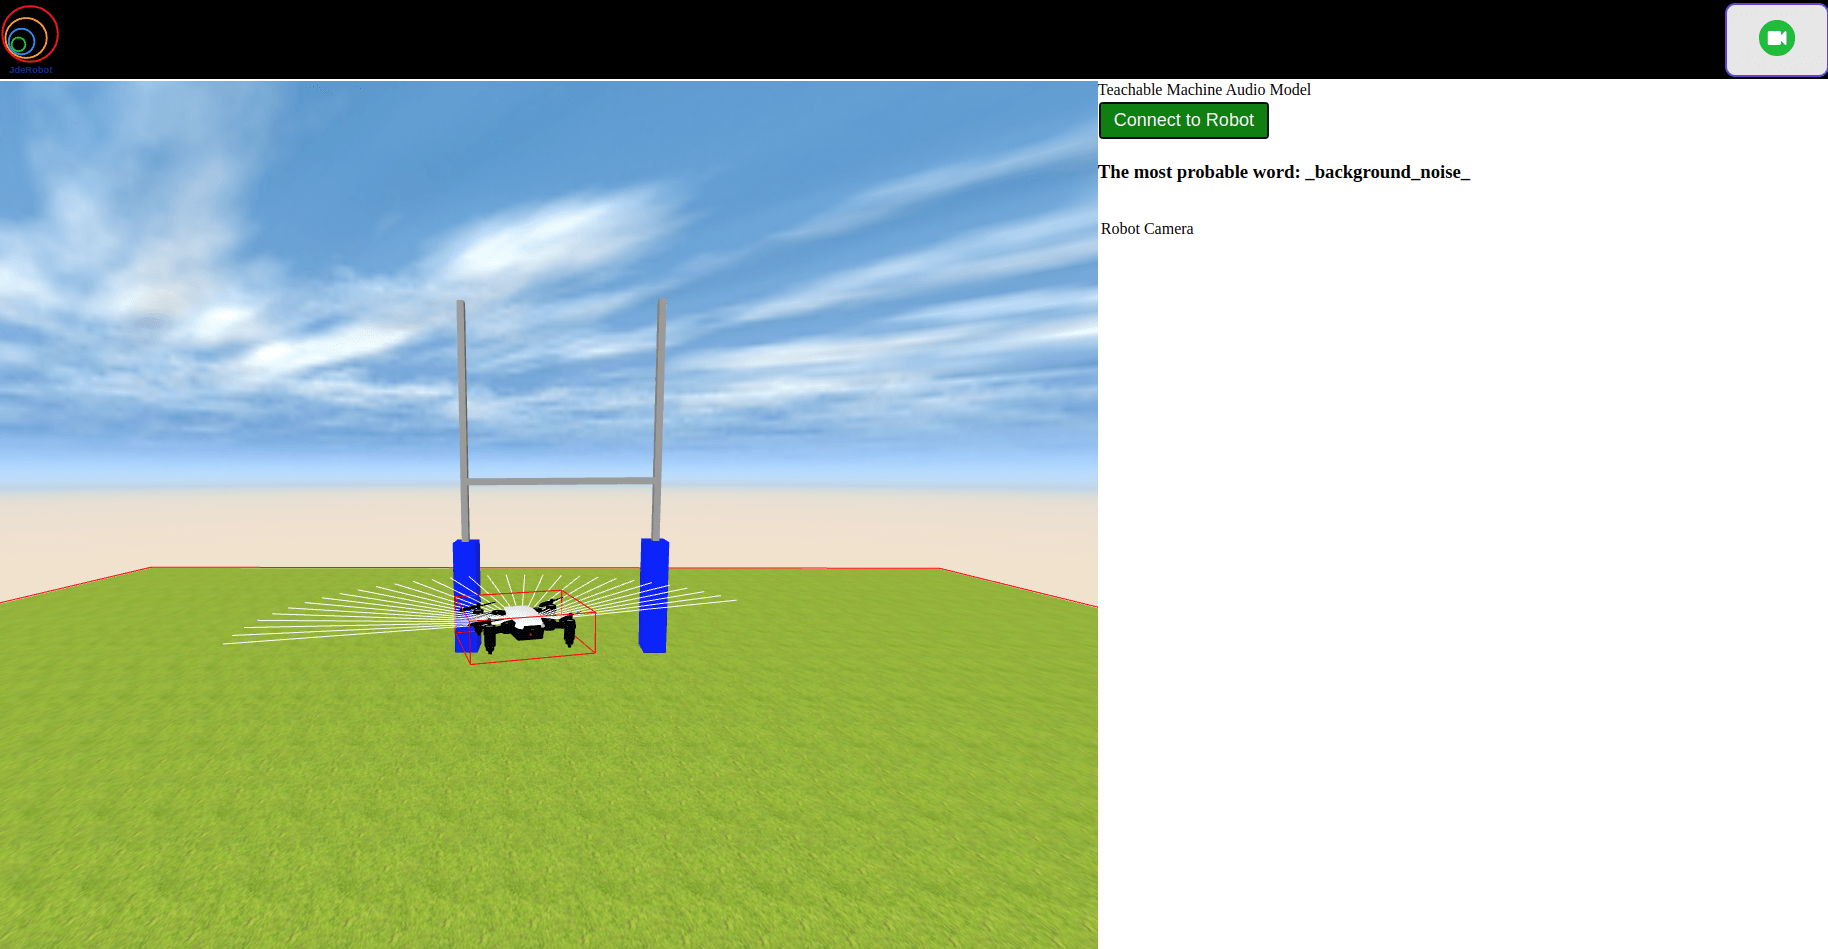
\includegraphics[width=0.8\textwidth, height=0.4\textwidth]{chapters/images/audio.png}
    \caption{Ejercicio teleoperador acústico}
    \label{fig:my_label}
\end{figure}

Cuando se pulsa el botón \textit{Conect\_To\_Robot} se llama a la función del mismo nombre que internamente ejecuta  la función \textit{listen()}  inicializa el reconocimiento y analiza el audio cada 10 segundos.
Este botón se pone en verde cuando está analizando y en rojo cuando está desconectado, mientras el bóton esté de ese color el robot no reconoce ninguna palabra.

La función \textit{listen()} inicializa el modelo y crea las etiquetas que necesita. Se ha creado un \textit{setTimeout} para esperar 10 segundos hasta que cargue el modelo. Cuando éste carga, se establece un \textit{setInterval} para que cada 10 segundos se ejecute la función \textit{analizar()} que devuelve la palabra estimada.

La función\textit{analizar()} es la que invoca al analizador o \textit{recognizer}: en él se predice la palabra que cree que es más probable que haya dicho el usuario.  \textit{Prediction} es esa palabra que tiene  la probabilidad más alta.

Una vez tenemos la \textit{prediction} se compara esta palabra con las 8 palabras que hemos entrenado el modelo: \textit{go, stop, back, right, left, up, down y \_background\_noise\_}

Gracias al evento \textit{'robot-loaded'}, cuando el robot está cargado en el escenario, obtenemos el objeto \textit{localRobot}, que en nuestro ejercicio es el dron. Kibotics ofrece una API\footnote{Application Programming Interfaces} llamada HAL API \footnote{Hardware Abstraction Layer} con funciones para controlar el movimiento del robot simulado. Cuando se predice una de las 8 palabras, en los condicionales \textit{if(){} else if() {}} se llama a una de estas funciones de velocidad : \textit{localRobot.setV()}, para asignar la velocidad lineal: se utiliza para ir hacia delante ``go'', ir hacia atrás ``back '' o parar ``stop''.  \textit{LocalRobot.setW()} para la velocidad angular: se usa para girar a la derecha``right'' o a la izquierda``left''. Y \textit{localRobot.setL()} para asignar la velocidad de subida y bajada: subir ``up'' o bajar ``down''. Si se predice que es ruido de fondo no afecta en el comportamiento del dron.

La implementación del ejercicio con Teachable Machine  nos ha aportado sencillez y más precisión que otros modelos que se estudiaron.
Una vez realizado el ejercicio se optimizó para que el navegador del usuario no estuviera todo el tiempo analizando el  audio si no tenemos nada que decirle al dron y aprovechar mejor así los recursos del ordenador del usuario.

La optimización se realizó añadiendo el contador \textit{(noise\_times)} que aparece en el código anterior: éste cuenta las veces que se predice ruido de fondo. Se estableció un máximo de 10 las veces seguidas que la predicción es \textit{\_background\_noise\_}. Como se analiza el audio cada 10 segundos, ésto quiere decir que si han pasado 100 segundos y siempre ha detectado ruido de fondo, la función \textit{analizar()} para de ejecutarse y no se predice ninguna palabra. Cuando ésto ocurre, se muestra en el navegador un nuevo botón \textit{(Continue analizing)} que al pulsarlo desaparece y se reinicia el procesamiento de audio. Ver Figura 6.7.

\begin{figure}[H]
  \begin{subfigure}[b]{0.5\textwidth}
  \centering
    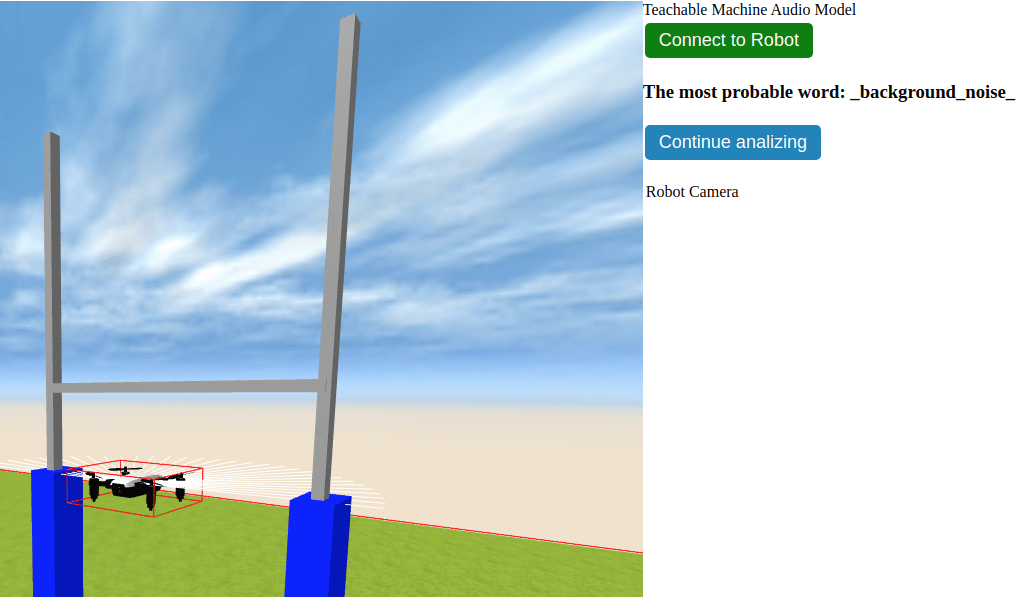
\includegraphics[width=0.95\textwidth, height=0.7\textwidth]{chapters/images/optimizacionaudio.png}
    \caption{Botón Continue analizing }
    \label{fig:f1}
  \end{subfigure}
  \hfill
  \begin{subfigure}[b]{0.5\textwidth}
  \centering
    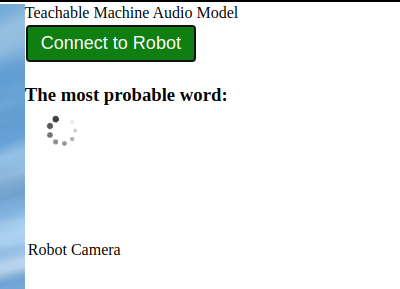
\includegraphics[width=0.95\textwidth, height=0.7\textwidth]{chapters/images/optimizacionaudio2.png}
	\caption{Se reinicia el procesamiento de audio.}    
    \label{fig:f2}
 
  \end{subfigure}
  \caption{Optimización del modelo }
\end{figure}




\section{Solución de referencia}

Este ejercicio es un juego, el objetivo es dirigir al dron con tu voz para cruzar por la portería de rugby o pasar de un lado al otro de la pared sin chocarte con ellas. Se ha realizado un vídeo promocional \footnote{https://youtu.be/sr54MxMw954} y este otro vídeo \footnote{https://www.youtube.com/watch?v=85oTxgQQrck} donde se muestran unas posibles soluciones para guiar al dron en los distintos escenarios. Ver Figura 6.8.

 \begin{figure}[H]
  \begin{subfigure}[b]{0.5\textwidth}
  \centering
    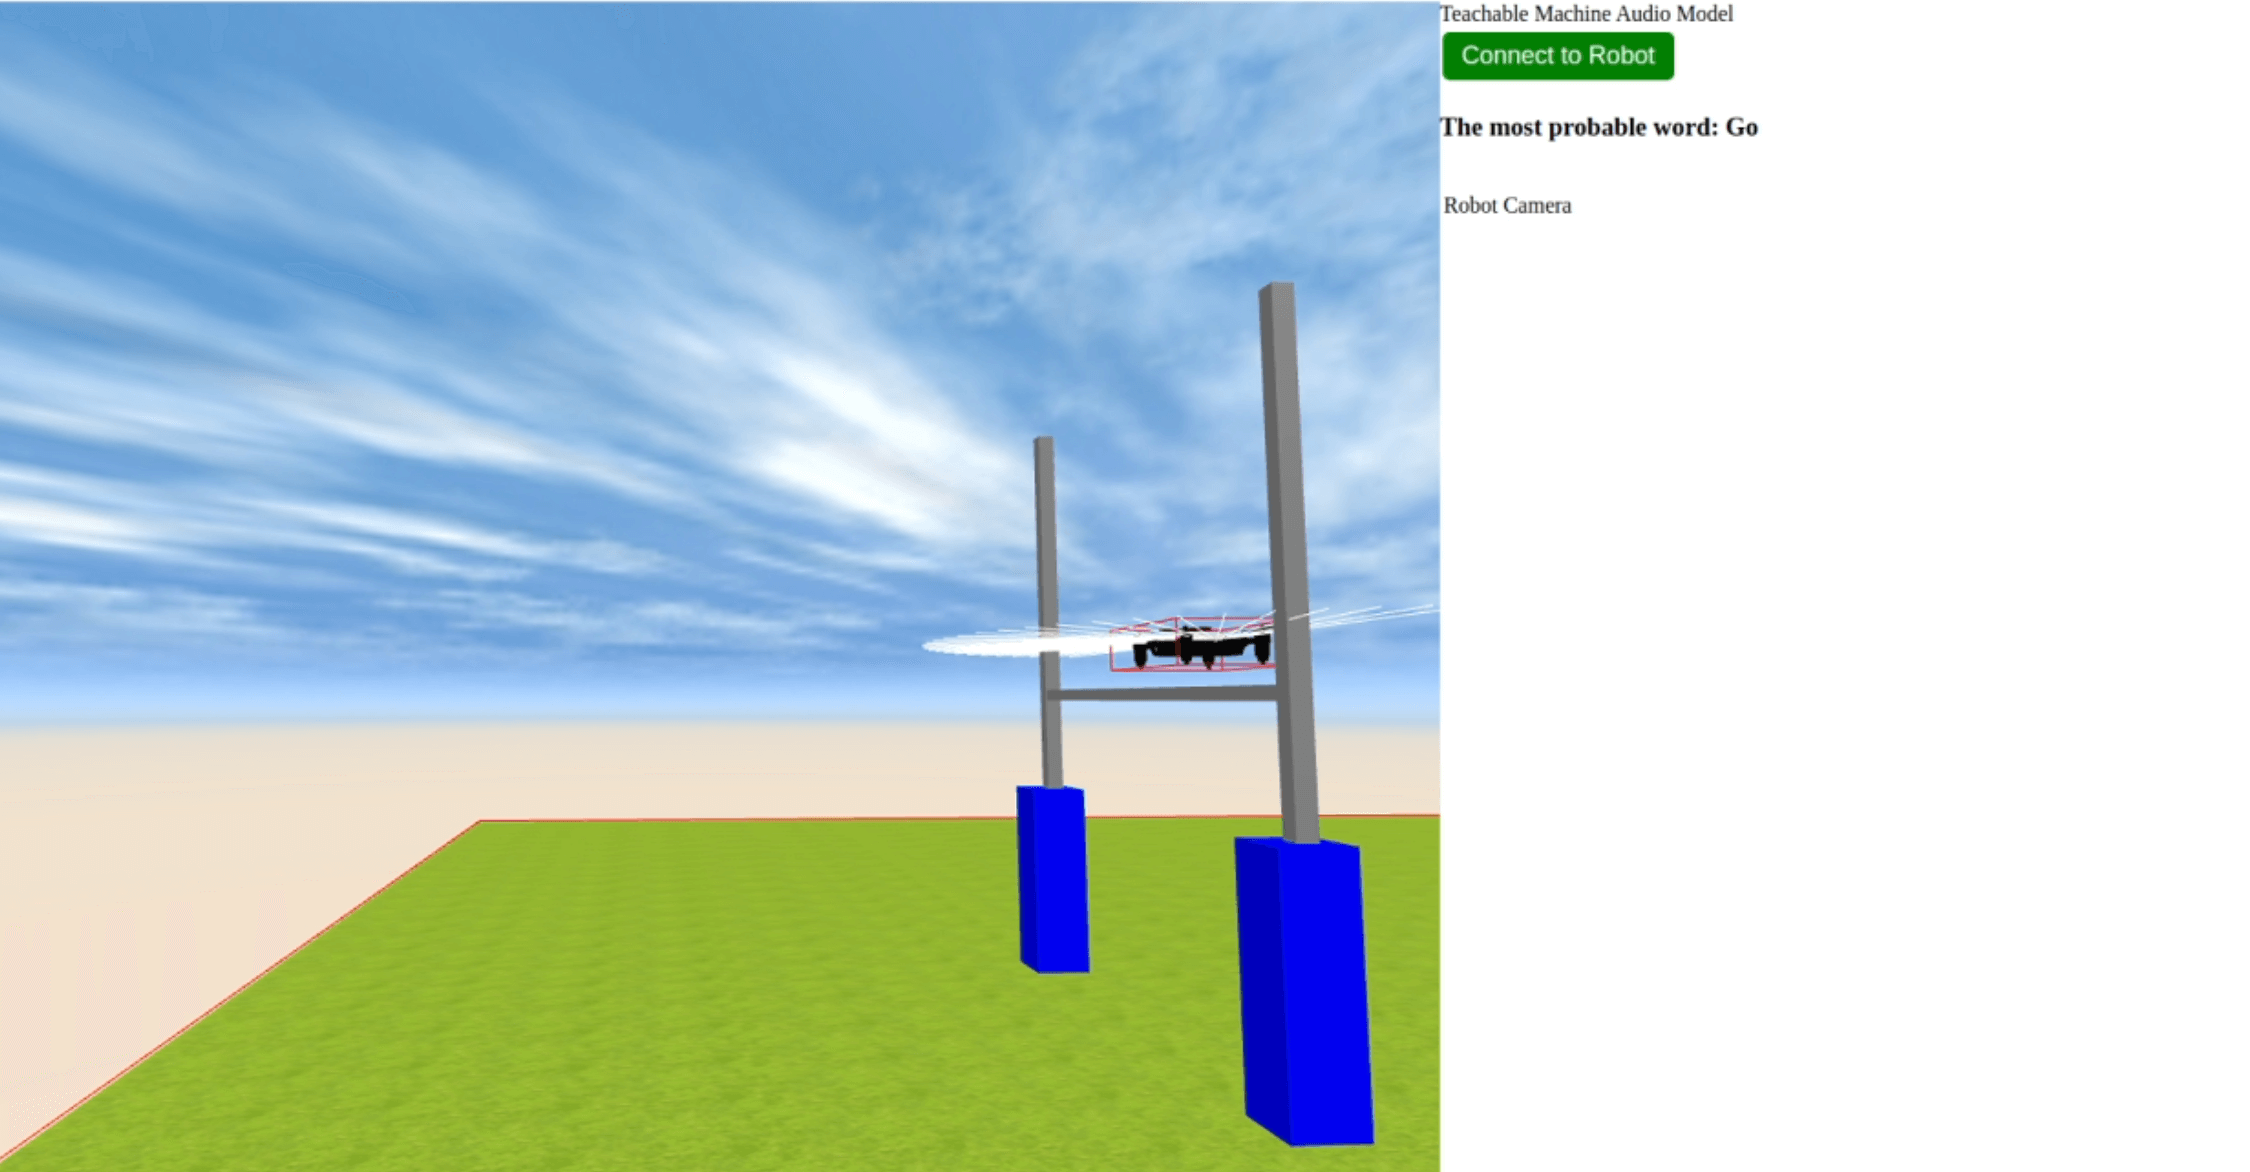
\includegraphics[width=1\textwidth, height=0.7\textwidth]{chapters/images/solucionaudio.png}
    \caption{}
    \label{fig:f1}
  \end{subfigure}
  \hfill
  \begin{subfigure}[b]{0.5\textwidth}
  \centering
    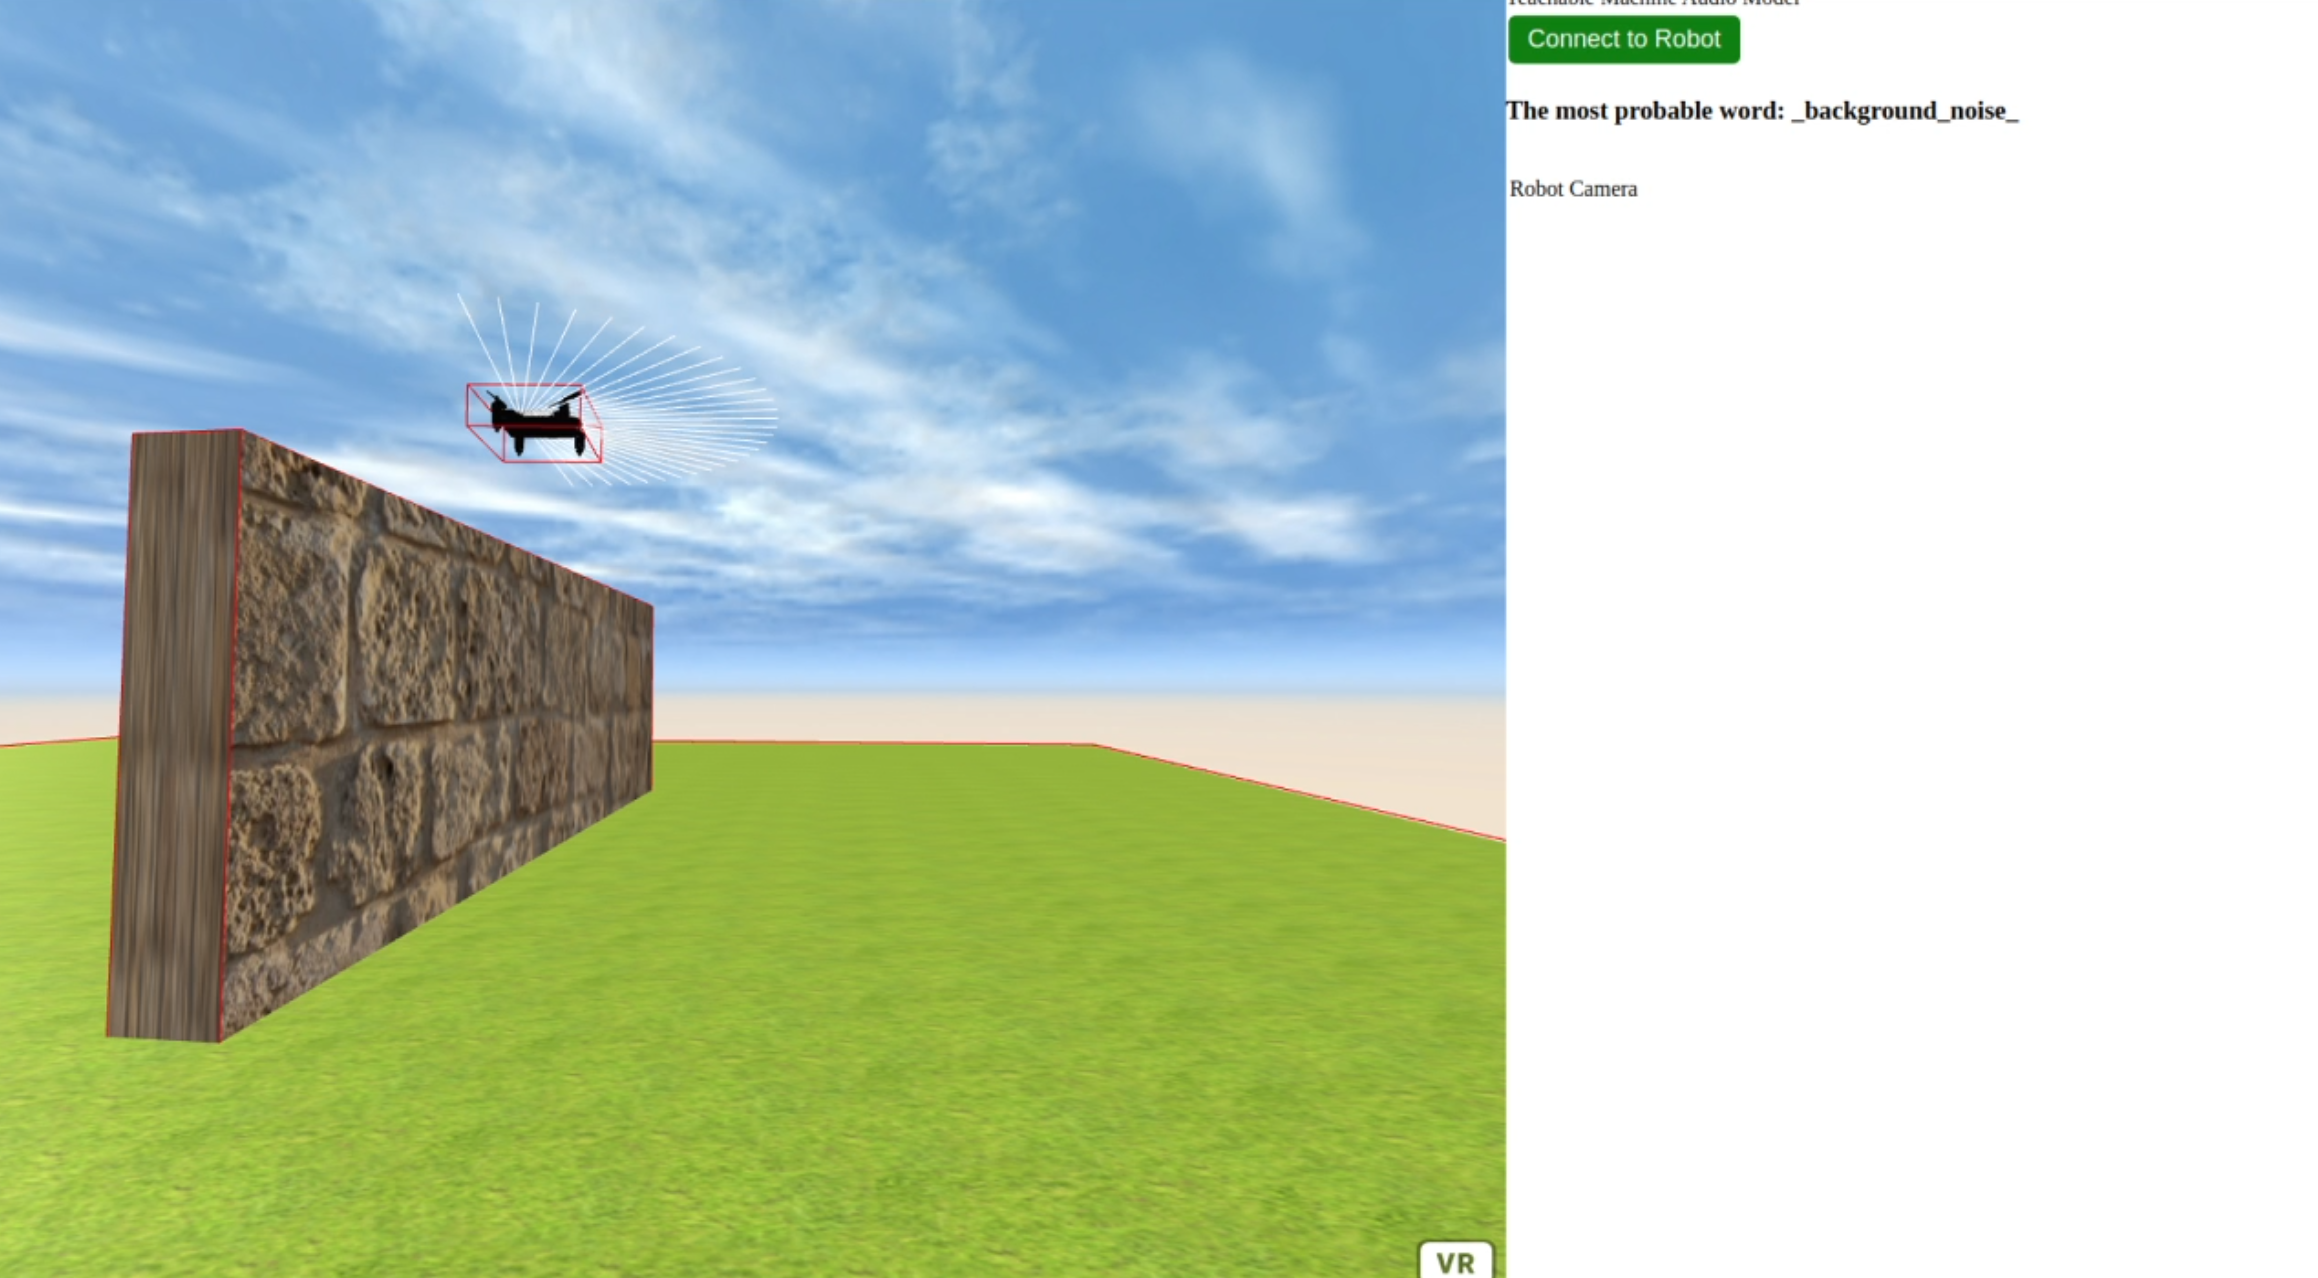
\includegraphics[width=1\textwidth, height=0.7\textwidth]{chapters/images/solucionaudio2.png}
	\caption{}    
    \label{fig:f2}
 
  \end{subfigure}
  \caption{Ejemplo solución teleoperador acústico}
\end{figure}


\section{Alternativas probadas}

Para llevar a cabo este ejercicio se estudiaron otras dos herramientas de procesamiento de audio además de Teachable Machine: Web Audio API y TensorFlow JS.

Web Audio API permite escoger fuentes de audio, agregar efectos de sonido, crear visualizaciones, efectos espaciales, filtros y grabaciones, entre otras cosas.
Se ha estudiado la  posibilidad de hacer una red neuronal con esta API. Con esta tecnología, en este TFG se hizo un grabador donde el audio se grababa temporalmente en la memoria del navegador y un analizador en frecuencia en tiempo real \cite{waa} .  En estos vídeos se puede ver el grabador \footnote{https://www.youtube.com/watch?v=u9aerlWpCdM} y el analizador \footnote{https://www.youtube.com/watch?v=OZk4l7WFTZw} mencionados.

Web Audio API es muy útil para visualizado y efectos de sonido pero no nos proporcionaba la suficiente información para poder hacer procesamiento de audio y reconocer palabras.

TensorFlow JS es una biblioteca de JavaScript para el aprendizaje automático. Esta herramienta se utiliza para clasificación de imágenes, detección de objetos, segmentación del cuerpo, estimación de pose, detección de rostros y, entre otras, aplicaciones de reconocimiento y clasificación de comandos de voz \cite{tensorflowmodel}.

Para empezar a entender cómo funcionan los modelos, capas y  tensores, en definitiva,  las redes neuronales en esta biblioteca, se realizaron distintos tutoriales de Youtube y de TensorFlow JS tanto de clasificación de imágenes como de reconocimiento de audio. En este video \footnote{https://www.youtube.com/watch?v=x8sUG1CyLdc} se ven las diferentes pruebas que se hicieron. En la Figura 6.9 se puede ver un ejemplo de modelo de detección de objetos.

\begin{figure}[H]
    \centering
    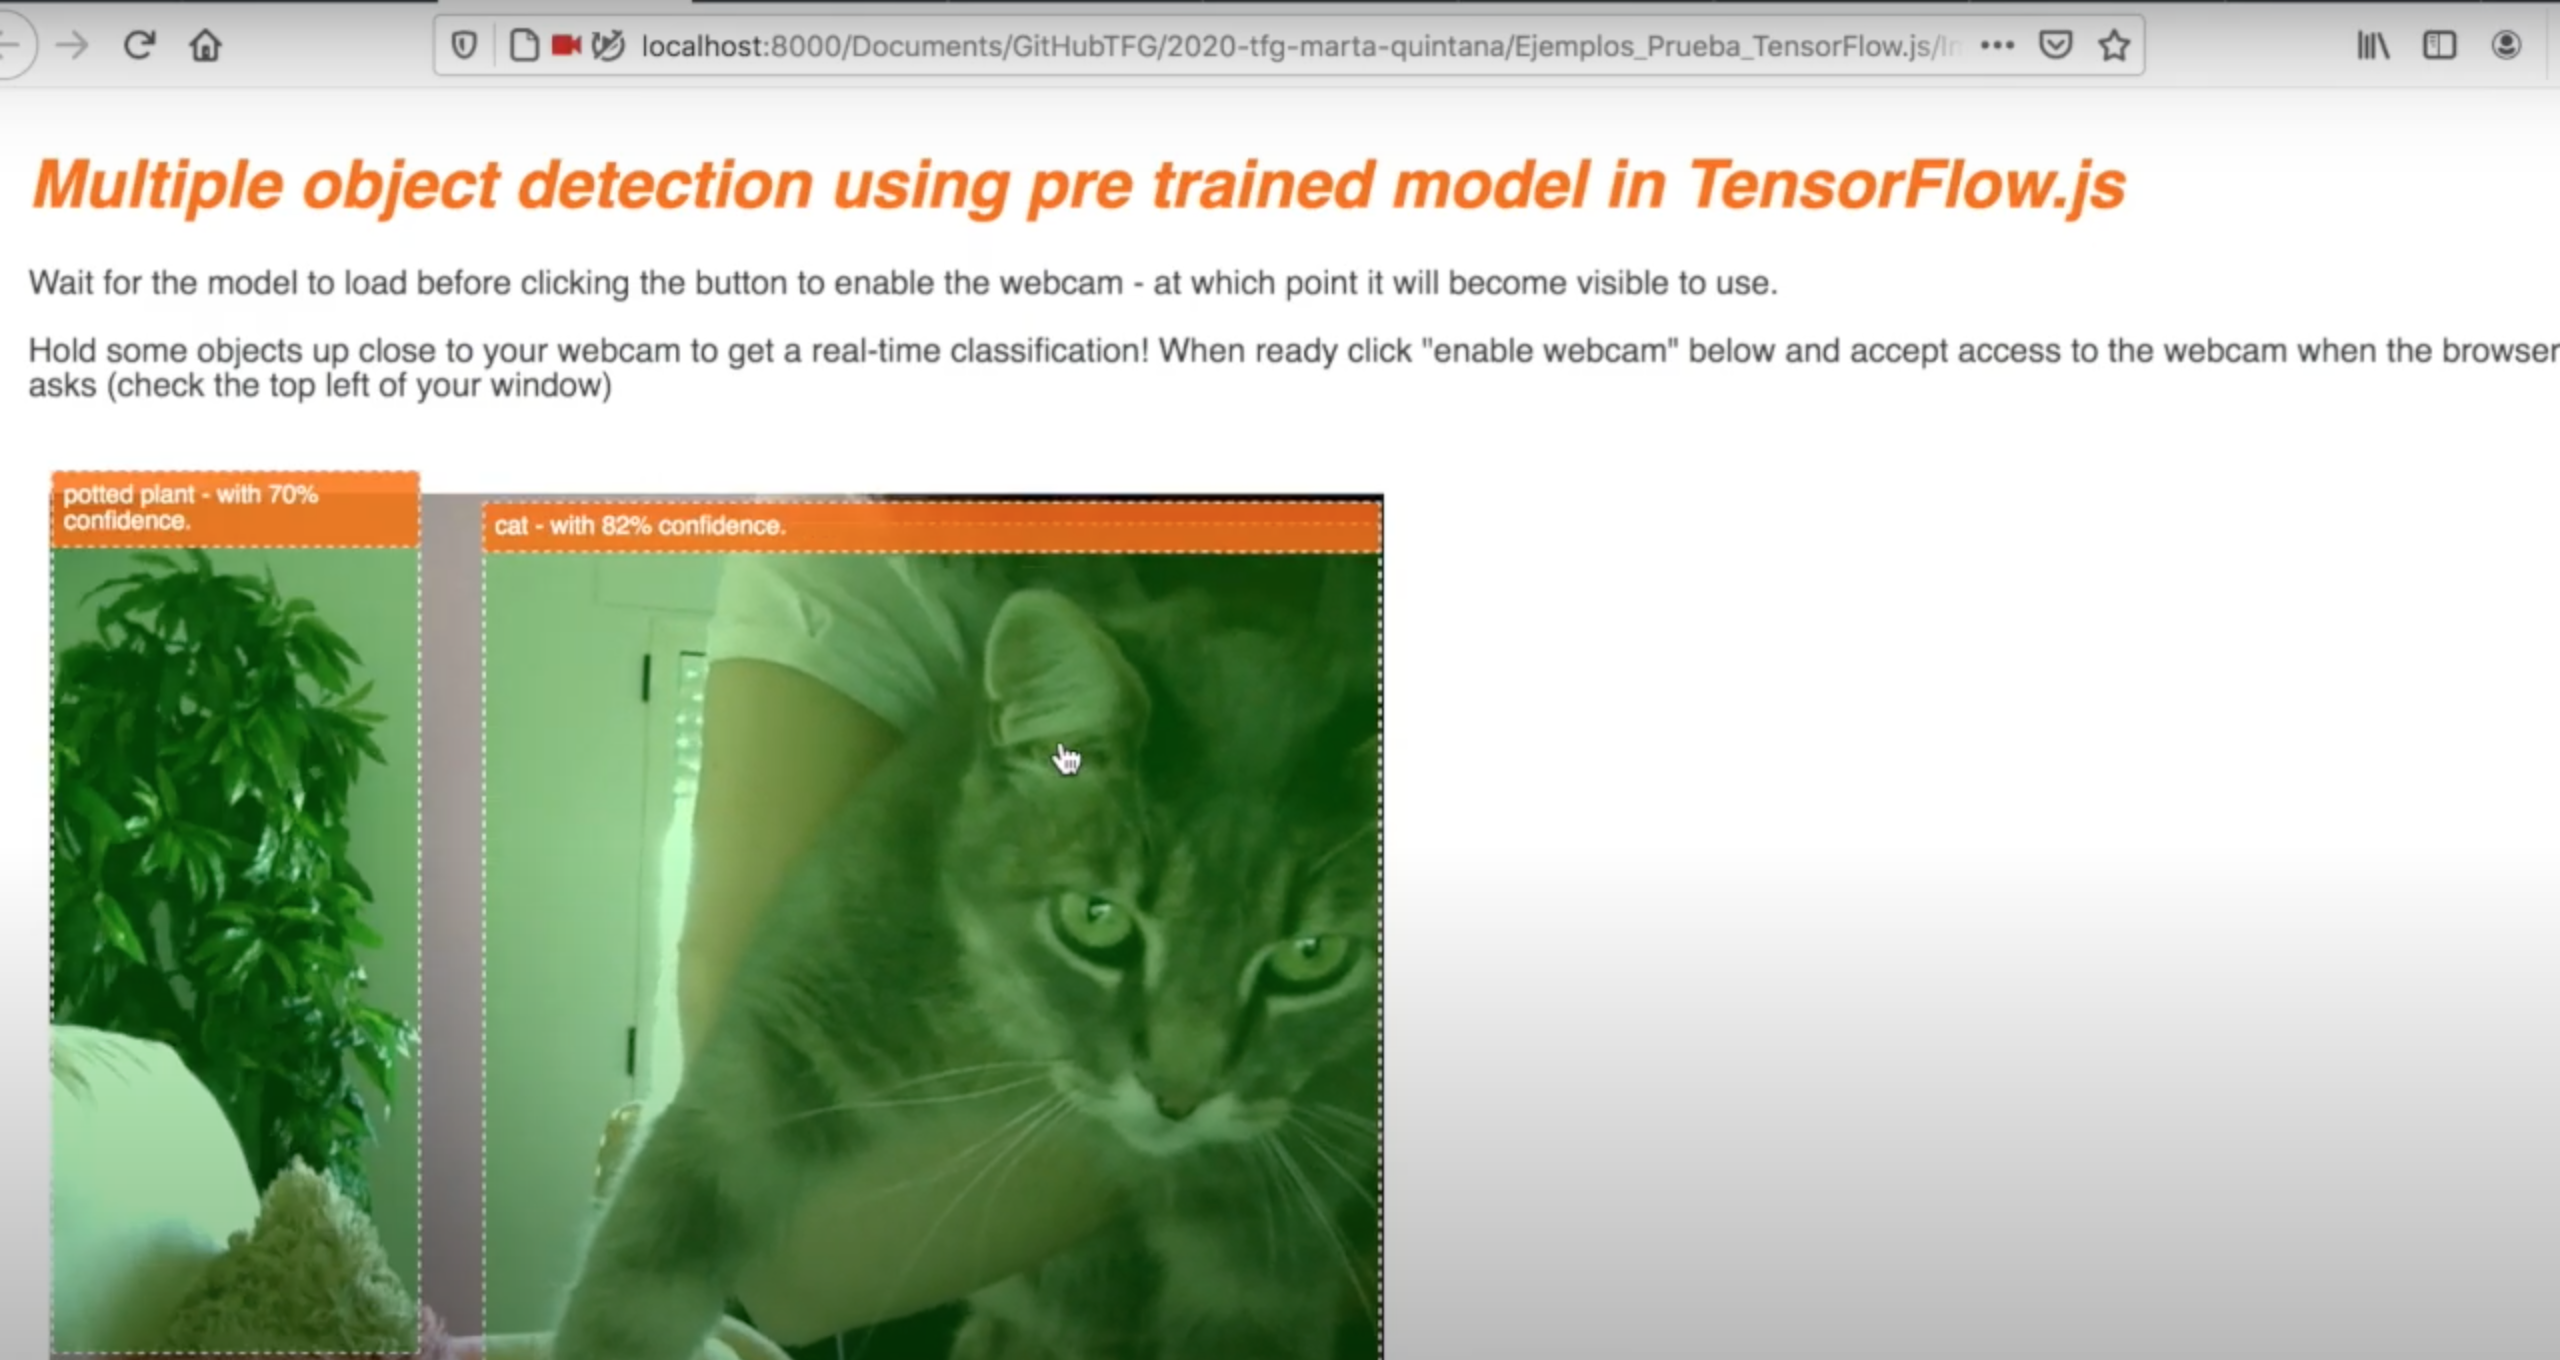
\includegraphics[width=0.8\textwidth, height=0.4\textwidth]{chapters/images/imagerecognition.png}
    \caption{TensorFlow JS ejemplo detección de objetos. }
    \label{fig:my_label}
\end{figure}

Con TensorFlow JS se hicieron dos prototipos. El primero se realizó con un modelo pre-entrenado que reconocía 10 palabras entre ellas \textit{go, stop, right, left y seven} (que se utilizó para que el robot fuera hacia atrás).
Este modelo al ser pre-entrenado y definido por TensorFlow JS no era muy exacto y el ruido de fondo afectaba demasiado a la hora de detectar cada palabra en nuestro ejercicio. Por ello, el segundo prototipo se hizo con un modelo que se entrenaba con la voz del usuario del ejercicio.

En este segundo prototipo cada palabra necesitaba grabar sus muestras, al menos unas 100 muestras por palabra, incluidas las muestras de ruido de fondo para que la detección fuera más precisa. Este modelo funcionaba más o menos bien pero no era lo más adecuado para el ejercicio que se había planteado. A pesar de que funcionaba bien se descartó porque era una tarea muy laboriosa grabar todas las muestras cada vez que entrabas en el ejercicio. 
En estos videos \footnote{https://www.youtube.com/watch?v=DcwJzCOE4kI}
\footnote{https://www.youtube.com/watch?v=nPeCAb47jiU} se puede ver cómo era el modelo.

Investigando el mundo de reconocimiento de audio y JavaScript se descubrió Teachable Machine, la tecnología que finalmente se ha elegido en este proyecto.


\section{Banda Sonora}

Para añadir banda sonora a los ejercicios existentes en Kibotics, se estudió cómo insertar audio desde HTML5 e implementarlo con JavaScript en Websim.

El elemento HTML \textless audio\textgreater  se usa para reproducir un fichero de audio en una página web.
Los atributos que destacan de este elemento son \textit{controls, source, loop y autoplay }.
El atributo \textit{controls} proporciona controles como reproducir, parar y subir o bajar el volumen.
 \textit{Source} permite especificar la fuente de audio, en este caso un fichero en formato mp3, ogg o wav. \textit{Loop} permite volver a reproducir el audio automáticamente cuando se termine, de esta forma  el audio estará en bucle. Y \textit{autoplay} se utiliza para que una vez se cargue el fichero de audio, éste empiece a reproducirse.

Para hacer esta mejora a Kibotics, en la carpeta \textit{assets} de Websim se añadió una nueva carpeta llamada \textit{``soundtracks''} con temas musicales para poner en los ejercicios. Las canciones usadas son de Patrick De Artega Royalty Free Music  \footnote{ https://patrickdearteaga.com Credits to Patrick De Artega Royalty Free Music 2020}
y los temas que se han añadido son:
Chiptronical, Common Fight, Goliath's Foe, Resilience, Spring Village, TheTrueStory of Beelzebub y Vals de su jardín.


La banda sonora de cada ejercicio se define en su fichero de configuración. En ese fichero se ha creado un objeto con la etiqueta ``soundtrack'', el identificador ``audio'' y la dirección del fichero fuente del audio (\textit{src}) que se quiere asignar como banda sonora, como se muestra en el siguiente código:

\begin{lstlisting}
 	{"tag":"soundtrack",
        "attr": {
            "id":"audio",
            "src": "../assets/soundtracks/Spring_Village.ogg"
          }
        },
   \end{lstlisting}

Websim tiene un analizador de ficheros json llamado config\_parser.js, con este fichero JavaScript se analiza el fichero de configuración (incluyendo el objeto que hemos mencionado anteriormente) y lo traduce a A-Frame. Se ha mejorado este analizador ficheros de Websim para materializar la banda sonora de cada ejercicio si está configurada.

Cuando Websim lee el fichero de configuración (formato JSON) se llama a \textit{parseSoundtrack()} que recibe los objetos de la escena para analizar si hay banda sonora o no en el ejercicio.

\begin{lstlisting}
 	await parseSoundtrack(sceneObjects);
\end{lstlisting}

En el siguiente código se muestra cómo se analizan todos los objetos de la escena. Si algún objeto tiene la etiqueta ``soundtrack'', una variable también llamada \textit{soundtrack}, que por defecto siempre es \textit{false}, pasa a ser \textit{true} y se asigna a la variable \textit{audio} el atributo  ``src'' del objeto,  que en este caso es  ``../assets/soundtracks/Spring\_Village.ogg".  
Si soundtrack es \textit{true}, se crea un objeto Audio() de HTML5 desde JavaScript y se le asigna el \textit{src} del la variable \textit{audio} y se empieza a reproducir. Como \textit{reproducir.loop} es \textit{true}, el audio estará en bucle todo el tiempo.

\begin{lstlisting}
export function parseSoundtrack(sceneObjects){
  var soundtrack = false;
  for (var i = 0; i <sceneObjects.length;i++){
   if (sceneObjects[i]['tag']== 'soundtrack'){
     soundtrack = true;
     var audio=sceneObjects[i]['attr']['src'];
    }
  }
  if (soundtrack) {
    var reproducir = new Audio();
        reproducir.src= audio
        reproducir.loop= true;
        reproducir.play();
  }
  return;
}
\end{lstlisting}

En este video \footnote{https://www.youtube.com/watch?v=c\_\_BayBCSX4} se puede escuchar la banda sonora que se ha asignado a un ejercicio de ejemplo.

\subsection{Efecto de sonido por colisión }

Los efectos de sonido son muy importantes en los juegos, es por ello que se pensó mejorar la experiencia del usuario añadiendo el efecto de sonido de colisión. 

Se implementó con el evento \textit{`collide'} de A-Frame. Cuando se detecta una colisión este evento llama a una función que reproduce un audio y pone a 0 todas las velocidades V, W y L del robot.  En este caso la reproducción del audio se hace una única vez por choque como pasaría en la realidad.

\begin{lstlisting}
  document.addEventListener('collide', function (e) {
      console.log('Robot has collided!');
      var reproducir = new Audio();
      reproducir.src= 'http://sonidosmp3gratis.com/sounds/000215403\_prev.mp3';   //collision sound
      reproducir.play();
      localRobot.setV(0);
      localRobot.setW(0);
      localRobot.setL(0);
	});
	
\end{lstlisting}

Esta función sirve para todos los ejercicios de la plataforma con o sin  bandas sonoras y para el teleoperador acústico. En el video de las soluciones  \footnote{https://www.youtube.com/watch?v=85oTxgQQrck}  en el escenario de la pared de piedra se puede escuchar el efecto de sonido por colisión cuando el dron choca con la pared.